\documentclass[
	xcolor=dvipsnames,
	aspectratio=169,	
	10pt, 
	]{beamer}
\graphicspath{{./fig/}}
\RequirePackage{"./sty/UserPackageManager"}
\usepackage{changepage}
%% TUBS
  \usebackgroundtemplate%
{
	
\includegraphics[width=\paperwidth,height=\paperheight]{./bonos/Bonobono}%
}
\setbeamercolor{section page}{fg = white}
\setbeamertemplate{section page}
{
	\begin{centering}
		\vfill
		\usebeamercolor[fg]{section page}
			\usebeamerfont{section title}\Huge \insertsection\par
		\vfill
	\end{centering}
}

\AtBeginSection[] % show section page automatically
{
	\begin{frame}
		\sectionpage
	\end{frame}
}
\setbeamertemplate{section in toc}{\Large \inserttocsectionnumber.~\inserttocsection}
\setbeamertemplate{subsection in toc}{\hspace{1.2em} $\bullet$~\inserttocsubsection}
\setbeamercolor{section in toc}{fg=white}
\setbeamercolor{subsection in toc}{fg=white}
\usepackage{biblatex}
\bibliography{Bibilography.bib}
\title[]{Notes on Kinematic Fit}
\author[Author]{Bono Bono}
\institute{Bono University}
\date{\today}
\subtitle{Bono, Bono\footnotemark[1]\newline\today}


\begin{document}

%%%%%%%%%%%%%%% Title page 
\begin{frame}[t,plain] % Cover slide
       \titlepage
        \footnotetext[1]{Bono University}
\end{frame}
\begin{frame}{Outline}
	\tableofcontents
\end{frame}
\section{Introduction}
\begin{frame}{Measurement Error}	
	\tcl{8}{8}{
		\begin{figure}
			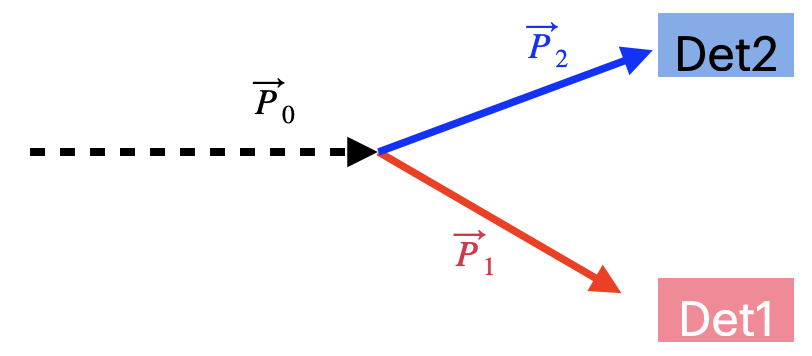
\includegraphics[width=.9\textwidth]{TwoBodyDecay}
		\end{figure}
	}{
	\begin{block}{}
		\large
		Assume a beam with momentum $\vec P^-$ decays into $\vec P_1$ and $\vec P_2$. Measured momentum are smeared due to detector resolution, leading to unbalance in the momentum conservation.
		\begin{align}
			\vec P_{0}=\vec P_{1}+\vec P_{2};\quad \vec P_{1,meas} + \vec P_{2,meas}\neq \vec P_{0} 
		\end{align}
		
	\end{block}
	}
	\begin{block}{}
		\large
	We can define the $\chi^2$ to quantitatively represent our measurement error. However, we can't derive meaningful expressions from this $\chi^2$. 
	\begin{align}
		\chi^2= \frac{(P_{1}-P_{1,meas})^2}{\sigma_1^2}+\frac{(P_{2}-P_{2,meas})^2}{\sigma_2^2}\label{chi2}
	\end{align}
	\end{block}
\end{frame}
\begin{frame}{Constrained Optimization with The Lagrange Multiplier}
	\begin{block}{}
		By incorporating the \textit{Kinematic Constraints}, specifically \textit{momentum conservation}, we involve additional knowledge to \eqref{chi2}. This is known as the \textit{Lagrange Multiplier}
		\begin{align}
			\chi^2= \frac{(P_{1,KF}-P_{1,meas})^2}{\sigma_1^2}+\frac{(P_{2,KF}-P_{2,meas})^2}{\sigma_2^2} + 2\mathbf{\lambda(P_{1,KF}+P_{2,KF}-P_0)}\label{LagMulti}
		\end{align} 
		Now we have meaningful expressions to minimize $\chi^2$, hence get better estimations for the measurement.
		\begin{align}
			\frac{1}{2}\pdf{\chi2}{P_{1,KF}}&=\frac{(P_{1,KF}-P_{1,meas})}{\sigma_1^2}+\lambda=0\label{dxd1}\\
			\frac{1}{2}\pdf{\chi2}{P_{2,KF}}&=\frac{(P_{2,KF}-P_{2,meas})}{\sigma_2^2}+\lambda=0\label{dxd2}
			\\
			\frac{1}{2}\pdf{\chi2}{\lambda}&=(P_{1,KF}+P_{2,KF}-P_0)=0\label{dxdl}
		\end{align}
	\end{block}
\end{frame}
\begin{frame}{Why Better Resolution?}
	\begin{block}{}
		By solving the equations \ref{dxd1},\ref{dxd2},\ref{dxdl} and defining $\delta_i = P_{i,meas} - P_i$, we obtain the following expressions:
		\begin{align}
			\lambda&=\frac{P_{1,meas}+P_{2,meas}-P_0}{\sigma_1^2+\sigma_2^2} = \frac{\delta_1 + \delta_2}{\sigma_1^2+\sigma_2^2}\\
			P_{1,KF}&=P_{1,meas}-\sigma_1^2\lambda\\
			P_{2,KF}&=P_{2,meas}-\sigma_2^2\lambda
		\end{align}
		\begin{align}
		<P_{1,KF}-P_{1}>& =<P_{1,KF}-P_{1,meas}+\delta_{1}>  = <-\sigma_1^2\lambda+\delta_1>\nonumber\\
		&=<\frac{-\sigma_1^2}{\sigma_1^2+\sigma_2^2}(\delta_{1}+\delta_{2})+\delta_1>=<\frac{\sigma_2^2\delta_1 -\sigma_1^2\delta_2}{\sigma_1^2+\sigma_2^2}> \\
		\sigma_{1,KF}^2 &= <(P_{1,KF}- P_1)^2> =\frac{\sigma_2^4\cancelto{\sigma_1^2}{<\delta_1^2>}+\sigma_1^4\cancelto{\sigma_2^2}{<\delta_2^2>}}{(\sigma_1^2+\sigma_2^2)^2} = \frac{\sigma_1^2\sigma_2^2}{\sigma_1^2+\sigma_2^2}<\sigma_1^2
	\end{align}
	\end{block}
\end{frame}
\begin{frame}{The Covariance After Kinematic Fit}
	\begin{block}{}
		\begin{align}
			cov(P_{1},P_{2})_{KF}& = <\delta_{1,KF}\delta_{2,KF}> = <(\delta_1 -\sigma_1^2\lambda)(\delta_2-\sigma_2^2\lambda)> \nonumber\\
			&= \sigma_1^2\sigma_2^2\cancelto{\frac{1}{\sigma_1^2+\sigma_2^2}}{<\lambda^2>}\quad -\quad \frac{\sigma_1^2<\delta_2^2>+\sigma_2^2<\delta_1^2>}{\sigma_1^2+\sigma_2^2} =-\frac{\sigma_1^2\sigma_2^2}{\sigma_1^2+\sigma_2^2}
		\end{align}
		\begin{align}
			V=\begin{pmatrix}
				\sigma_1^2&0\\
				0&\sigma_2^2
			\end{pmatrix}\to V_{KF} =
			\begin{pmatrix}
\frac{\sigma_1^2\sigma_2^2}{\sigma_1^2+\sigma_2^2}&-\frac{\sigma_1^2\sigma_2^2}{\sigma_1^2+\sigma_2^2}\\
-\frac{\sigma_1^2\sigma_2^2}{\sigma_1^2+\sigma_2^2}&\frac{\sigma_1^2\sigma_2^2}{\sigma_1^2+\sigma_2^2}
			\end{pmatrix}
		\end{align}
		\begin{itemize}
			\item Improved momentum resolution
			\item Negative correlation between $P_1$ and $P_2$
		\end{itemize}
	\end{block}
\end{frame}
\begin{frame}{Generalization to Multi-Variables}
	\begin{block}{}
		Assume that we have a set of measured data $\mathbf{m^0}$, unknown parameters $\mathbf {u^0}$ and constraints $\mathbf f^0$.
		\begin{align}
			\mathbf {m^0} =\{m_1^0,m_2^0\ldots m_N^0\};\quad \mathbf {u^0} =\{u_1^0,u_2^0\ldots u_J^0\}\nonumber\\
			\mathbf f =\{f_1(m_1^0,m_2^0,\ldots m_N^0,u_1^0,u_2^0,\ldots u_N^0),f_2^0,\ldots f_K^0\}
		\end{align}
		 Let $\mathbf m^0$ denote our initial measured data, and $\mathbf m$ represent the 'guess' of the data in each iterative step, just alike $P_{KF}$s in the previous example. Equation \eqref{LagMulti} is generalized to:
		\begin{align}
			\chi^2(\mathbf{m}) = (\mathbf{m}^0-\mathbf{m})^\dagger V^{-1}(\mathbf{m}^0-\mathbf{m})+2\mathbf\lambda^\dagger \mathbf {f}(\mathbf{m,u}).\label{KFChi2}
		\end{align}
		Here, the Lagrange multiplier $\mathbf \lambda =\{\lambda_1,\lambda_2,\ldots\lambda_K\}$ is not just a number but a column vector with k elements, corresponding to each kinematic constraint in $\mathbf f$. 
	\end{block}
\end{frame}

\begin{frame}{$\chi^2$ Minimization}
	\begin{block}{}
		We want to solve the equation
		\begin{align}
			\vec \nabla \chi^2 =0
		\end{align}
		to obtain the minimized state. The differential term are listed within three groups.
		\begin{align}
			\nabla_{\mathbf m} &= -2 V^{-1}(\mathbf m^0)(\mathbf m^0-\mathbf m) + 2 \mathbf F_\mathbf m^\dagger(\mathbf{m,u})\mathbf\lambda=0\label{GradM}\\
			\nabla_{\mathbf u} &= 2\mathbf F_\mathbf u^\dagger(\mathbf{m,u})\mathbf \lambda =0\label{GradU}\\
			\nabla_{\mathbf \lambda}& = \mathbf f(\mathbf{m,u})\label{GradL}.
		\end{align}
		Here, the subscripts denote partial derivatives. i.e. ($(\mathbf {F}_m)_{ki}\equiv\pdf {f_k}{m_i}$).
	\end{block}
	\begin{block}{User Should Define...}
		\begin{table}
			\begin{tabular}{c|c|c|c}
				$\mathbf{m}$&$\mathbf{u}$&$\mathbf{f}$&$\mathbf{V}$\\\hline
				Measured Data&Unknown parameters&Constraints&Covariance Matrix
			\end{tabular}
		\end{table}
	\end{block}
\end{frame}
\section{Example: Mass-Constraint Fit}
\begin{frame}{Example: $\Lambda\to p\pi$, Defining Variables and Constraints}
	\begin{block}{}
		Assume a decay of $\Lambda\to p\pi^-$. We define the measurements and unknowns as:
		\begin{align}
			\mathbf{m}=\{P_p,\theta_p,\phi_p,P_\pi,\theta_\pi,\phi_\pi\};\quad\mathbf{u} = \{P_\Lambda,\theta_\Lambda,\phi_\Lambda\}
		\end{align}
		Then we define the energy-momentum constraint equation as:
		\begin{align}
			\begin{pmatrix}
				f_1\\f_2\\f_3\\f_4
			\end{pmatrix}=
			\begin{pmatrix}
				-P_\Lambda\sin\theta_\Lambda\cos\phi_\Lambda+P_p\sin\theta_p\cos\phi_p+P_\pi\sin\theta_\pi\cos\phi_\pi\\
				-P_\Lambda\sin\theta_\Lambda\sin\phi_\Lambda+P_p\sin\theta_p\sin\phi_p+P_\pi\sin\theta_\pi\sin\phi_\pi\\
				-P_\Lambda\cos\theta_\Lambda+P_p\cos\theta_p+p_\pi\cos\theta_\pi\\
				-\sqrt{P_\Lambda^2+m_\Lambda^2}+\sqrt{P_p^2+m_p^2}+\sqrt{P_\pi^2+m_\pi^2}
			\end{pmatrix}.\label{FMat}
		\end{align}
		where the mass constraint is naturally implemented in energy term.
		
		Since we have 3 unmeasured variable with 4 kinematical constraints, this is a 4-3 = 1-Constrained fit.
	\end{block}
\end{frame}
\begin{frame}{Example: $\Lambda\to p\pi$, The Derivatives}
	\begin{block}{}
		 We get $\mathbf{F_u}$ and $\mathbf{F_m}$ as
		\begin{align}
			\mathbf{F_u}=
			\begin{pmatrix}
				\pdf{f_1}{P_\Lambda}&\pdf{f_1}{\theta_\Lambda}&\pdf{f_1}{\phi_\Lambda}\\
				\pdf{f_2}{P_\Lambda}&\pdf{f_2}{\theta_\Lambda}&\pdf{f_2}{\phi_\Lambda}\\
				\pdf{f_3}{P_\Lambda}&\pdf{f_3}{\theta_\Lambda}&\pdf{f_3}{\phi_\Lambda}\\
				\pdf{f_4}{P_\Lambda}&\pdf{f_4}{\theta_\Lambda}&\pdf{f_4}{\phi_\Lambda}
			\end{pmatrix};\quad \mathbf{F_m}=\begin{pmatrix}
				\pdf{f_1}{P_p} &\cdots&\pdf{f_1}{\phi_\pi} \\
				\pdf{f_2}{P_p} &\cdots&\pdf{f_2}{\phi_\pi}\\
				\pdf{f_3}{P_p} &\cdots&\pdf{f_3}{\phi_\pi}\\
				\pdf{f_4}{P_p} &\cdots&\pdf{f_4}{\phi_\pi}
			\end{pmatrix}
		\end{align}
		We have all the matrices to calculate in each step. By applying an appropriate variance matrix and employing $\chi^2$ selection criteria, we can do kinematic fit for the particles.
	\end{block}
\end{frame}
\begin{frame}{Example: $\Xi\to \Lambda\pi$, $\Lambda\to p\pi$}
	\begin{block}{}
		We require two mass constraints for $\Xi\to \Lambda\pi;\quad \Lambda\to p\pi$. In this case, careful considerations on the selection of variables. We will select
		\begin{align}
			\mathbf{u} = \{P_\Xi,\theta_\Xi,\phi_\Xi\};\quad \mathbf{m}=\{P_p,\theta_p,\phi_p,P_\pi,\theta_\pi,\phi_\pi\}
		\end{align}
		and define five constraints as:
		\begin{align}
			\begin{pmatrix}
				f_1\\f_2\\f_3\\f_4\\f_5
			\end{pmatrix}=
			\begin{pmatrix}
				-P_{\Xi,x}+P_{p,x}+P_{{\pi_\Lambda},x}+P_{{\pi_\Xi},x}\\
				-P_{\Xi,y}+P_{p,y}+P_{{\pi_\Lambda},y}+P_{{\pi_\Xi},y}\\
				-P_{\Xi,z}+P_{p,z}+P_{{\pi_\Lambda},z}+P_{{\pi_\Xi},z}\\
				-E_\Lambda +E_p+E_{\pi_\Lambda}\\
				-E_\Lambda +E_p+E_{\pi_\Lambda}+E_{\pi_\Xi}
			\end{pmatrix}.
		\end{align}
		$\Lambda$ variables are not selected in $\mathbf u$ to avoid negative DoF.($N_{f} - N_{u} = 5 - 6 = -1$)
			
		Note that \textbf{we don't have explicit terms} related to $\vec P_\Lambda$, i.e.  $-P_{\Lambda,x}+P_{p,x}+P_{{\pi_\Lambda},x}$ etc., because $\vec P_\Lambda$ are neither unmeasured nor measured variables in our choice of parameters.  
	\end{block}
\end{frame}
\section{Example: $\Xi $ decay at J-PARC}
\section{Tricks}
\begin{frame}{Off-diagonal Reduction}
	content...
\end{frame}
\begin{frame}{Parameter Normalization}
	content...
\end{frame}
\section{Calculations}
\begin{frame}{Processing Iterative Steps.}
	\begin{block}{}
		We can express the following equations based on the ones provided above:
		\begin{align}
			&V^{-1}(\mathbf m^0)(\mathbf{m}^{\nu+1}-\mathbf{m}^0)+(\mathbf{F}_m^\dagger)^\nu\mathbf\lambda^{\nu+1}=0\label{DelM}\\
			&(\mathbf{F}_u^\dagger)^\nu\mathbf\lambda^{\nu+1}=0\label{DelU}\\
			&\mathbf f^\nu + \mathbf F^\nu_m (\mathbf m^{\nu+1}-\mathbf m^\nu) + \mathbf F^\nu_u(\mathbf u^{\nu+1}-\mathbf u^\nu)=0\label{DelL}.
		\end{align}
		Equation \eqref{DelL} is not a direct consequence of Equation \eqref{GradU} but rather a \textit{linear approximation} to proceed with our iteration step. Expanding the $\nabla_\lambda$ term with a Taylor series leads to this equation. 
		Note that, as our parameters $\mathbf m$ and $\mathbf u$ are updated during the step, our constraint matrix $\mathbf f$ should also be updated during the iteration. Here, $\lambda$ should be indexed as $\nu+1$ since it is a parameter to be guessed in the next step.
	\end{block}
\end{frame}

\begin{frame}{Solving the Equation(1)}
	\begin{block}{}
		Multiplying \textbf V to Equation \eqref{DelM} leads to:		\vspace{-2 mm}
		\begin{align}
			\mathbf{m}^{\nu+1}-\mathbf{m}^0=-V(\mathbf m^0)(\mathbf{F}_m^\dagger)^\nu\mathbf\lambda^{\nu+1}.\label{Mnu}
		\end{align}
		Substituting Equation \eqref{Mnu} into Equation \eqref{DelL}, we get:\vspace{-2 mm}
		\begin{align}
			\mathbf F^\nu_u(\mathbf u^{\nu+1}-\mathbf u^\nu) &= - \mathbf f^\nu - \mathbf F^\nu_m (-V(\mathbf m^0)(\mathbf{F}_m^\dagger)^\nu\mathbf\lambda^{\nu+1} +\mathbf{m}^0-\mathbf{m}^\nu  )\nonumber\\
			&=  S\lambda^{\nu+1}  - R\label{SLambda}
		\end{align}
		where$S\equiv \mathbf{F}_\mathbf{m}^\nu V(\mathbf m^0)(\mathbf{F}_\mathbf{m}^\dagger )^\nu$  and $R\equiv \mathbf f^\nu + \mathbf{F}_\mathbf{m}^\nu(\mathbf{m}^0-\mathbf{m}^\nu)$. Multiplying $(\mathbf{F}_u^\dagger)^\nu S^{-1}$ and substituting Equation \eqref{DelU}, we get:\vspace{-2 mm}
		\begin{align}
			(\mathbf{F}_u^\dagger)^\nu S^{-1}\mathbf F^\nu_u(\mathbf u^{\nu+1}-\mathbf u^\nu) = \ctz{(\mathbf F_u^\dagger)^\nu\mathbf \lambda^{\nu+1}}-(\mathbf{F}_u^\dagger)^\nu S^{-1}R.
		\end{align}
	\end{block}
\end{frame}
\begin{frame}{Solving the Equation(2)}
	\begin{block}{}
		Then we naturally obtain:
		\begin{align}
			\mathbf{u}^{\nu+1}=\mathbf{u}^\nu - ((\mathbf{F}_u^\dagger)^\nu S^{-1}\mathbf F^\nu_u)^{-1}(\mathbf{F}_u^\dagger)^\nu S^{-1}R\label{Unu}.
		\end{align} 
		and from Equation \eqref{SLambda}
		\begin{align}
			\mathbf\lambda^{\nu+1} = S^{-1}(\mathbf F^\nu_u(\mathbf u^{\nu+1}-\mathbf u^\nu) + R)\label{Lnu}
		\end{align}.
		For a summary, we have obtained all equations to proceed to the next step. All other matrices in the equation can be calculated from parameters of the current step, and $\chi^2$ can be evaluated from \eqref{KFChi2} .
		\begin{align*}
			\begin{cases}
				\mathbf{u}^{\nu+1}=\mathbf{u}^\nu - ((\mathbf{F}_u^\dagger)^\nu S^{-1}\mathbf F^\nu_u)^{-1}(\mathbf{F}_u^\dagger)^\nu S^{-1}R&\eqref{Unu}\\
				\mathbf\lambda^{\nu+1} = S^{-1}(\mathbf F^\nu_u(\mathbf u^{\nu+1}-\mathbf u^\nu) + R)&\eqref{Lnu}\\
				\mathbf{m}^{\nu+1}=\mathbf{m}^0-V(\mathbf m^0)(\mathbf{F}_m^\dagger)^\nu\mathbf\lambda^{\nu+1}&\eqref{Mnu}
			\end{cases}
		\end{align*}
	\end{block}
\end{frame}
\begin{frame}{Evolution of the Variance Matrix}
	\begin{block}{}
		Take a look at Eq.\eqref{Mnu}. We see that $m^{\nu+1} $ is an addition(subtraction) of some parameters to the initially measured data. As we already know the error, i.e. Variance matrix, of initial data, we can estimate how error propagates through the fitting process. 
		\begin{align}
			V(m) = J_{m,m^0}V(m^0)J_{m,m^0}^\dagger
		\end{align}
		We need to calculate the Jacobian, 
		\begin{align}
			J_{m,m^0(i,j)} = \pdf{m_i}{m^0_j}
		\end{align}
	\end{block}
\end{frame}
\begin{frame}{Evolution of the Variance Matrix.}
	\begin{block}{}
		To begin with, let us express Eq \eqref{Mnu} in terms of $m^0$. At the moment we will drop the superscript $\nu$. As $\vecb f(\vecb m,\vecb u)$is a constant on $m^0$, $\vecb F_\vecb m$ also will be a constant to $m^0$. Then we only need to consider the derivatives of $\lambda$. By substituting \eqref{Unu} ,
		\begin{align}
	\mathbf\lambda = S^{-1}(-\mathbf F_u(((\mathbf{F}_u^\dagger) S^{-1}\mathbf F_u)^{-1}(\mathbf{F}_u^\dagger) S^{-1}R) + R)
		\end{align}
		and we have
		\begin{align}
			R\equiv \mathbf f + \mathbf{F}_\mathbf{m}(\mathbf{m}^0-\mathbf{m})\to \pdf{R}{m^0}= \vecb F_m
		\end{align} 
		so that 
		\begin{align}
			\pdf{\lambda}{m^0}= S^{-1}(-\mathbf F_u((\mathbf{F}_u^\dagger S^{-1}\mathbf F_u)^{-1}\mathbf{F}_u^\dagger S^{-1}\vecb F_m) + \vecb F_m).
		\end{align}
	\end{block}
\end{frame}
\begin{frame}{Evolution of the Variance Matrix}
	\begin{block}{}
		Now define the symmetric matrices $G\equiv \vecb {F_m^\dagger} S^{-1}\vecb {F_m}$, $U\equiv (\mathbf{F}_u^\dagger S^{-1}\mathbf F_u)^{-1}$ and $H\equiv \mathbf{F}_m^\dagger S^{-1}\vecb {F_u}$. Then we have expressions for $\pdf{\lambda}{m^0}$ hence 
		\begin{align}
			J_{m,m^0}&=I - V(m^0)\vecb{F}_m^\dagger\pdf\lambda{m^0}=I - V\vecb{F}^\dagger_m(-S^{-1}\vecb F_u U^{-1}H^\dagger+S^{-1}\vecb F_m)\nonumber\\
			&=I-V(G-HUH^\dagger)
		\end{align}
		If we let $C =G-HUH^\dagger$, we obtain
		\begin{align}
			V(m) = J_{m,m^0} VJ_{m,m^0}^\dagger =V -2 VCV  +VCVCV.\label{Vm}
		\end{align}
		You might want to neglect higher order term, but please keep 2nd order term at the moment. Some materials like \cite{Prob} had an error in this part.
	\end{block}
\end{frame}

\begin{frame}{Pull distribution}
	\begin{block}{}
		It is better to check the pull distribution to check the quality of a fit. By defining the residual $\epsilon = m-m^0$ and its variance $V(\epsilon)$, pull is defined as:, 
		\begin{align}
			P(\epsilon) = \epsilon/\sqrt{V(\epsilon)}
		\end{align}
		and
		\begin{align}
			V(\epsilon) \equiv V(m)+ V(m^0) - 2 Cov(m,m^0).\label{Ve}
		\end{align}
		We have already calculated $J_{m,m^0}$. Then we directly get the covariance matrix. 
	\end{block}
\end{frame} 
\begin{frame}{Pull distribution}
	\begin{block}{}
		The covariance can be estimated as:
		\begin{align}
			Cov(m,m^0) = J_{m,m^0}V(m) = V - VCV.
		\end{align}
		If we substitute this and Eq.\eqref{Vm} into Eq.\eqref{Ve}, we get
		\begin{align}
			V(\epsilon) = VCVCV.
		\end{align}
		Note that 2nd order term affects the variance.	
	\end{block}
\end{frame}
\begin{frame}{Variance of the Unknowns}
	\begin{block}{}
		Just like how we derived  Eq.\eqref{Vm} we can estimate the variance matrix of the unknowns. 
		\vspace{-3 mm}
		\begin{align}
			V_U = J_{u,m0} V J_{u,m0}^T
		\end{align}
		$J_{u,m0}$ can be obtained from Eq.\eqref{Unu}. Denoting\\ $((\mathbf{F}_u^\dagger)^\nu S^{-1}\mathbf F^\nu_u)^{-1}(\mathbf{F}_u^\dagger)^\nu S^{-1}$ as $K$, 
		\vspace{-3 mm}
		\begin{align}
			J_{u^{\nu+1},m^0} = \pdf {u^{\nu+1}} {m^0} = \pdf{u^{\nu}}{m^0} - K\pdf R {m^0} \simeq -K \vecb F_m.
		\end{align}
		Note that we only have initial "Guess" for the unknowns; In principle, it is not a driven value from measurements. Then, $\pdf {u^0}{m_0} = 0$. Also, we approximate that the terms in 2nd or higher iterations are negligible: $J_{u,m^0}\simeq J_{u^0,m^0}$.
	\end{block}
\end{frame}
\begin{frame}{Applications}

\end{frame}

\begin{frame}{Example: Chained Mass-Constraint Fit}
	content...
\end{frame}
\begin{frame}{Mass-Constraint Kinematic Fit with HypTPC.}
	\begin{block}{}
		\begin{figure}
			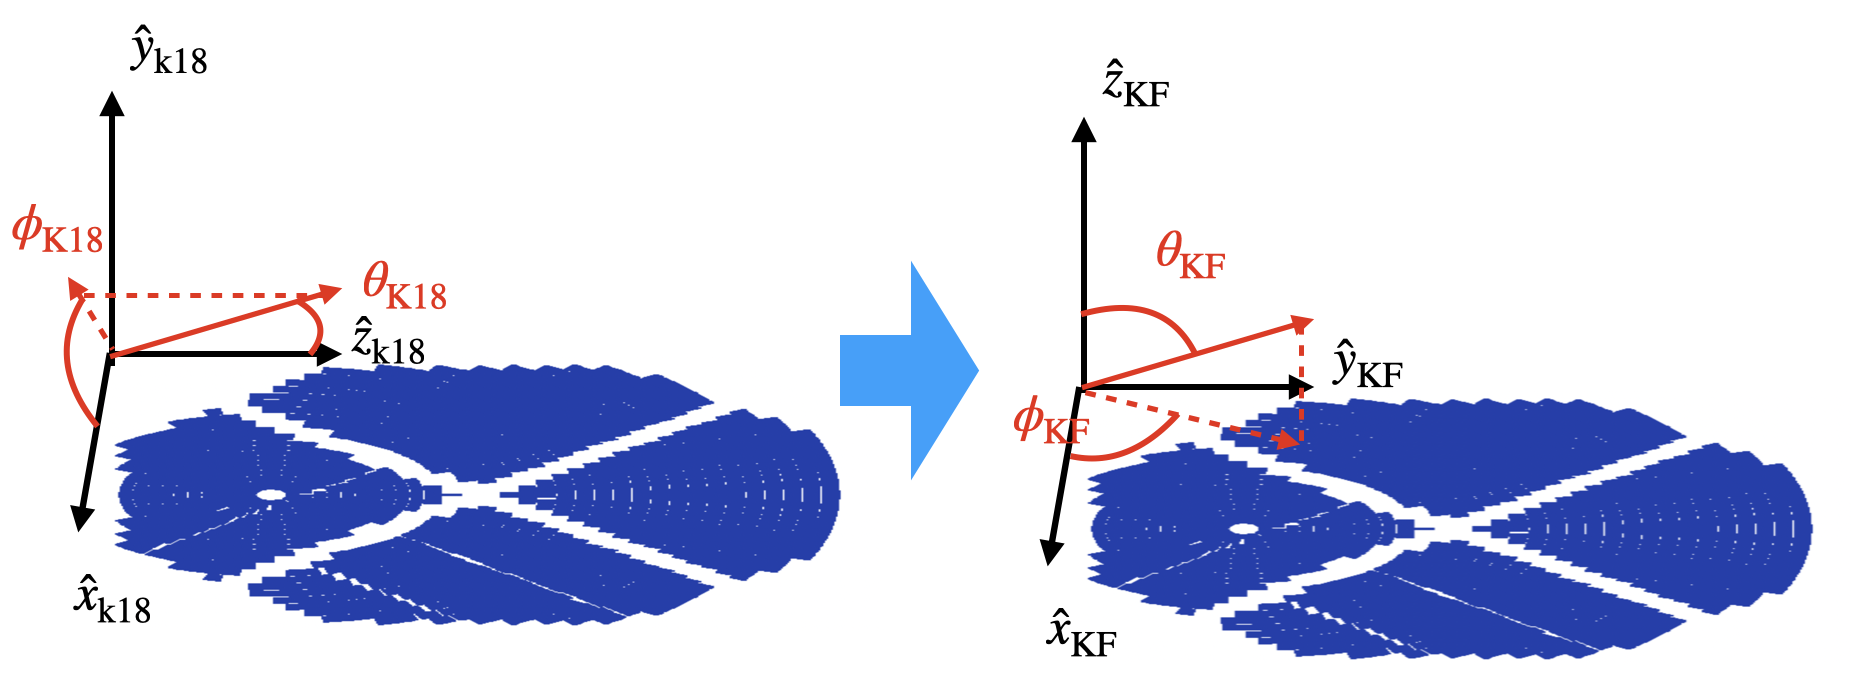
\includegraphics[width=0.9\textwidth]{Coords_K18_KF}
		\end{figure}
		For Kinematic FIt in HypTPC analysis, we want our coordinate system to be aligned with $\vec B$, so that our covariance matrix representation fits the representations in KF coordinate. We correlated $\phi$ angle with $p$ as an feature of helix fit, where $\phi$ is the angle lying on the circle of the helix. 
	\end{block}
\end{frame}
\iffalse
\begin{frame}{Estimating the Covariance in Helix Track}
	\begin{block}{}
		In many cases, we measure the momentum of reconstructed particles from their helical trajectories. The decay vertex is reconstructed from the intersection of two helix tracks, and the corresponding momentum direction is defined at the vertex of the helix. Since the transverse momentum is inversely proportional to the radius of the helical track, any deviation in momentum results in a corresponding deviation in the radius. As the radius increases or decreases, the tangent line at the intersection vertex rotates, leading to a strong correlation between the transverse momentum and the azimuth angle. Meanwhile, the zenith angle is defined from the pitch of the helix, which corresponds to the slope in arc-length vs $\Delta$ y of the spatial points used in helix fit.
	\end{block}
\end{frame}
\fi
\begin{frame}{Covariance Matrix in Helix Track}
	\begin{block}{}
	\tcl{3}{6}{
	\vspace{-7 mm}
	\begin{figure}
		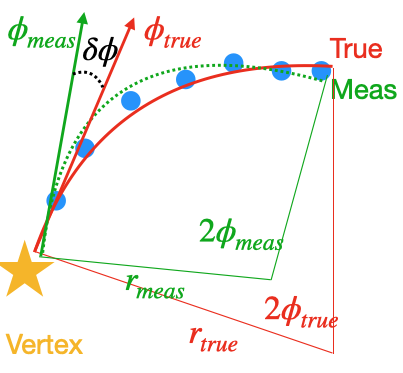
\includegraphics[width=4 cm]{PT_Phi}
	\end{figure}
}
{
	The cartoon on the left illustrates the correlation between the helical (or circular) track and the azimuth angle at the intersection point (or decay vertex). Since the helical trajectory is defined by measured spatial points, a deviation in radius does not shift the arc itself but moves the center of the circle. It is also worth noting that the arc length, $l$, remains nearly constant. 
}
If we let the azimuth angle at the center of the track as $\phi_0$, we deduce following relations:
\vspace{-4 mm}
\begin{align}
	\phi = \phi_0 \pm \frac{l}{2r};\quad  \delta\phi = \pm\frac{l}{2r}\frac{\delta r}{r}= \pm\frac{l}{r}\frac{\delta p_T}{p_T}
\end{align}
\vspace{-2 mm}
and we naturally obtain:
\vspace{-2 mm}
\begin{align}
	\sigma_{\phi}^2 = \langle\delta\phi\delta\phi\rangle=\frac{l^2}{r^2p_{T}^2}\sigma^2_{p_T};\quad \textrm{Cov}(\phi,p_T)= \langle\delta\phi\delta p_T \rangle = \pm \frac{l}{rp_T}\sigma_{p_T}^2
\end{align}
\end{block}
\end{frame}
\begin{frame}{Covariance Matrix in Helix Track}
	\begin{block}{}
			\tcl{3}{6}{
			\vspace{-7 mm}
			\begin{figure}
				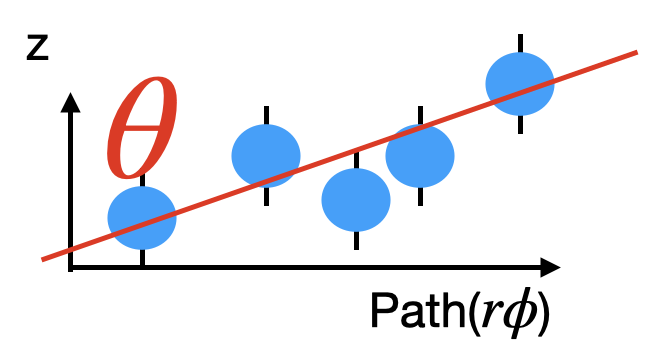
\includegraphics[width=4 cm]{Res_Th}
			\end{figure}
		}
		{
			The left figure illustrates the relationship between the pitch(dz) and the helix fit. The pitch is determined by fitting the vertical displacement along transverse path of the helical trajectory. Denoting the polar angle is expressed as 
		}
$\theta = \frac{\pi}{2}-\arctan(dz)$, we estimate the varaiance of $\theta$ based on the fitting error of dz, the slope parameter of linear fit.
		\begin{align*}
			\sigma_{dz}^2 =\frac{\sum\delta_z^2/(n-2) }{\sum(x-\bar x)^2} \simeq \frac{n \sigma_z^2/(n-2)}{n L^2/12};\quad \sigma_\theta = \pdf{dz}{\theta}\sigma_{dz}=\frac{1}{1+dz^2}\sigma_{dz}.
		\end{align*}
		Note that, the momentum $p_z=p_T dz$ would also have some covariance with $\theta$,
		\begin{align*}
			\langle \delta p\delta \theta\rangle = dz\langle  \ctz{\delta p_T  \delta \theta}\rangle+	p_T\langle \delta dz \delta \theta\rangle =\frac{p_T}{1+dz^2}\sigma_{dz}^2.
		\end{align*}
	
	\end{block}
\end{frame}
\begin{frame}{Example: MassVertex-Constraint Fit}
	\begin{block}{}
To be Updated..
	\end{block}
\end{frame}
%\begin{frame}[allowframebreaks]{References}
\begin{frame}{References}
	 	\printbibliography
\end{frame}
\end{document}
